\chapter{Background}\label{background}

Nel contesto delle moderne infrastrutture distribuite, il monitoraggio e la verifica di proprietà svolgono un ruolo cruciale nel garantire l'affidabilità, la sicurezza, il comportamento desiderato e le performance dei sistemi complessi.
Con l'evoluzione delle tecnologie come la virtualizzazione, la containerizzazione e l'adozione di architetture a microservizi, la necessità di soluzioni di monitoring efficaci è cresciuta esponenzialmente. Tali soluzioni devono essere in grado di raccogliere, analizzare e valutare dati provenienti da vari nodi distribuiti, al fine di mantenere la continuità operativa e prevenire eventuali guasti.
Questo capitolo esplora in dettaglio il concetto di monitoring nei sistemi distribuiti analizzando le principali \emph{proprietà non funzionali} e focalizzandosi sulle metodologie di \emph{Assurance} e \emph{Certification} basati su \emph{metriche, evidence e contratti}

Le tecniche di \textbf{assurance} sono finalizzate a garantire che un sistema rispetti, e quindi soddisfi, determinate \emph{proprietà non funzionali} precedentemente definite. \\
La \textbf{certification}, invece, consiste nel processo di verifica che attesta la conformità del sistema a requisiti specifici.

\section{Sistemi Distribuiti}
I paradigmi architetturali tradizionali si basano su un sistema centralizzato, caratterizzato da un singolo nodo centrale con cui tutti gli utenti interagiscono,
che coordina tutte le operazioni e fornisce dei servizi, tuttavia questa tipologia di architettura non è più in grado di soddisfare le esigenze del mercato odierno, richiedente elaborazione in tempo reale di grandi quantità di dati e interazione \textit{real-time} per un numero crescente di utenti.
Per cercare di soddisfare queste esigenze hanno avuto rapida diffusione i \emph{sistemi distribuiti}, caratterizzati dalla presenza di diversi nodi interconnessi,
non obbligatoriamente nello stesso luogo fisico, ma che operano come un'unica unità agli occhi dell'utilizzatore suddividendo così compiti e risorse.
Lo scopo di questi sistemi è gestire in modo efficiente le risorse a disposizione, elaborare rapidamente grosse quantità di dati e fornire agli utenti dei servizi.

I vantaggi nell'utilizzo di sistemi distribuiti risiedono nelle migliorie apportate ad affidabilità e prestazioni. Rispettivamente, non esiste più \emph{il singolo punto di errore} centrale ma vari nodi distribuiti (con anche repliche) pronti a sostituire il nodo guasto; mentre la seconda miglioria emerge dalla facilità con cui un sistema e i relativi nodi sono \emph{scalabili} sia orizzontalmente (creazione di altri nodi) che verticalmente (assegnazione di più risorse ad un nodo) andando così a mantenere stabili le prestazioni.
Questa architettura non solo migliora la scalabilità e l'affidabilità dell'applicazione, avendo diversi nodi distribuiti e sempre attivi,
ma offre anche una maggiore flessibilità e resilienza di fronte ai guasti.

I sistemi distribuiti, data la loro complessità realizzativa, richiedono di soddisfare determinate \emph{proprietà} per non vanificare gli sforzi implementativi e valorizzare l'impiego di questa architettura \cite{Tanenbaum_Distributed_Systems}. Tra questi abbiamo:
\begin{itemize}
	\item \emph{Accessibilità delle risorse}: un sistema distribuito deve, come obbiettivo primario, rendere le risorse remote facilmente accessibili e amministrarle in modo efficiente.
	\item \emph{Trasparenza}: un sistema distribuito deve nascondere il fatto che le risorse e i processi sono fisicamente distribuiti nella rete su vari sistemi, e deve presentarsi agli utenti come un'unica entità.
	\item \emph{Apertura}: un sistema distribuito deve offrire servizi fondati su regole standard che ne descrivono la sintassi e la semantica. I servizi offerti vengono specificati attraverso \textit{interfacce} definite con un \textit{Interface Definition Language} come OpenAPI\footnote{\url{https://openapi.it/}} (usato da Swagger\footnote{\url{https://swagger.io/}}).
	\item \emph{Scalabilità}: un sistema distribuito deve, in base alle esigenze, aumentare o diminuire le risorse e i nodi;  è la proprietà che differenzia in modo sostanziale un sistema distribuito da uno centralizzato e ne consente la facile evoluzione.
\end{itemize}

I \emph{sistemi distribuiti} vengono anche classificati in 3 macro-aree secondo \cite{Tanenbaum_Distributed_Systems}:
\begin{itemize}
	\item \emph{Computing systems} (sistemi di elaborazione): utilizzati per attività di elaborazione ad alte prestazioni; vedono il loro successo quando il rapporto prezzo/performance dei singoli dispositivi non diventa più accessibile ma conviene costruire un sistema componendolo.
	\item \emph{Information systems} (sistemi informativi): utilizzati in organizzazioni che possiedono una grossa quantità di applicazioni in rete per semplificarne l'interoperabilità tramite la comunicazione diretta delle varie componenti; questa procedura viene definita \textit{enterprise application integration}.
	\item \emph{Pervasive/embedded systems} (sistemi pervasivi/integrati): sono i sistemi caratterizzati da dispositivi piccoli, alimentati a batteria, mobili e con connessioni wireless, comunemente identificati come \textit{smartphones}. Un importante vantaggio di questi sistemi è l'assenza di supervisione amministrativa umana: i dispositivi devono scoprire automaticamente e autonomamente il contesto e ambientarsi per poter funzionare.
\end{itemize}

\subsection{Da sistemi monolitici a microservizi}\label{Da sistemi monolitici a microservizi}
Un sistema \textbf{centralizzato o monolitico,} modello tradizionale di deployment degli ultimi decenni, consiste in un applicativo software compilato come unica entità, autonoma e indipendente in grado di fornire dei servizi.
Lo stato è contenuto all'interno dell'unico nodo centrale. \\
Questo approccio, sebbene semplice da implementare e gestire inizialmente, presenta diversi limiti man mano che l'applicazione cresce in termini di dimensioni e complessità \cite{monolithic_to_microservices}; tra le principali limitazioni vengono identificate le seguenti:
\begin{itemize}
	\item \emph{Flessibilità e Scalabilità limitate}: le modifiche, sia funzionali che di scalabilità, devono essere apportate su tutto il sistema, essendo costituito da un'unica entità, e non sulla singola unità operativa che lo necessita.
	      I requisiti di prestazioni computazionali che una singola macchina dovrebbe soddisfare per permetterne un adeguato scaling verticale potrebbero risultare insoddisfacibili.
	\item \emph{Affidabilità limitata}: essendo il sistema costituito da un'unica entità, \textit{single-point-of-failure}, un singolo errore potrebbe compromettere l'intero sistema oppure fare da \textit{collo di bottiglia}
	\item \emph{Tempi di sviluppo e deployment lenti}: la natura monolitica impone di dover ricompilare e ridistribuire l'intera applicazione anche per piccole modifiche, rallentando il ciclo di sviluppo e rilascio.

\end{itemize}

La transizione da architetture monolitiche a \textbf{microservizi} rappresenta una delle evoluzioni più significative nel campo dello sviluppo software degli ultimi decenni segnando l'inizio del \gls{SOC}, il cui obbiettivo è usare i servizi come struttura base per costruire applicazioni \cite{SOC}. Questa trasformazione nasce dall'esigenza di trovare una soluzione alle restrizioni presenti nei precedenti modelli architetturali. \\
In un'architettura a microservizi, un'applicazione è suddivisa in una serie di servizi modulari indipendenti, ciascuno dei quali è responsabile di una specifica funzionalità e può essere sviluppato, distribuito e scalato in modo autonomo. Questa metodologia si integra perfettamente con il concetto di \emph{\gls{SaaS}} e come architettura modulare per componenti \gls{IoT}, garantendo guadagni in termini di performance, dinamismo e resilienza \cite{microservices_iot} \cite{microservices_in_iot}.
I vantaggi principali derivanti dall'adozione di questa architettura sono:
\begin{itemize}
	\item \emph{Scalabilità granulare}: ogni servizio può essere scalato indipendentemente dagli altri andando quindi ad ottimizzare l'utilizzo di risorse risultando in un complessivo aumento di performance
	\item \emph{Flessibilità nello sviluppo}: lo sviluppo rispecchia la struttura isolata dei vari applicativi permettendo manutenzioni separate per ogni servizio
	\item \emph{Ciclo di Sviluppo e Deployment rapidi}: ogni microservizio viene distribuito come entità indipendente dalle altre accelerando il rilascio di nuove funzionalità (\textit{continuous delivery})
	\item \emph{Rafforzamento dell'affidabilità}: i guasti sono strutturalmente isolati a livello di servizio riducendo le possibilità di blocco dell'intero sistema.
\end{itemize}

Le \emph{architetture a microservizi} sono diventate uno standard architetturale nello sviluppo di sistemi distribuiti e si integrano particolarmente bene a tecniche di \emph{continuous delivery} con periodici rilasci automatici, rientrando quindi nella categoria del \emph{DevOps} \cite{microservice_enable_devops}.
Vengono eseguiti maggiori rilasci di aggiornamenti grazie alla divisione delle componenti e alla possibilità di lavorare su singole parti dell'applicativo.

\subsection{Virtualizzazione e Container}
I sistemi distribuiti, caratterizzati dalla cooperazione di più nodi per eseguire compiti complessi, hanno guidato l'evoluzione verso tecnologie che ottimizzano l'efficienza e la scalabilità, come la virtualizzazione e la ``containerizzazione``.
La prima consente di sfruttare al massimo le risorse hardware, creando ambienti isolati che eseguono applicazioni in parallelo. La seconda, evoluzione del primo concetto, offre un livello di isolamento più leggero e rapido, permettendo una distribuzione agile delle applicazioni in ambienti distribuiti. La sinergia tra sistemi distribuiti e queste tecnologie è fondamentale per l'implementazione efficiente e scalabile di architetture moderne.

\paragraph{Virtualizzazione}
il processo di virtualizzazione consiste nel creare un livello di astrazione
sopra a quello fisico del sistema, rendendo così disponibili risorse in forma software e permettendo
la suddivisione del singolo sistema in molteplici virtuali con le rispettive risorse allocate. Il sistema
che ospita la virtualizzazione, comunemente identificato come “host”, condivide le proprie risorse hardware
con i molteplici sistemi software che ospita, comunemente identificati con “guests”.
Il software che viene utilizzato per raggiungere questo scopo è definito come “hypervisor”.
Ogni sistema virtuale viene creato in un ambiente di lavoro completamente isolato contenente
il sistema operativo, i file e le librerie necessarie; questa procedura provoca un overhead nel sistema
e richiede degli istanti di tempo prima che la macchina sia avviata ma dall'altro lato garantisce una
forte proprietà di isolazione: una violazione di sicurezza in un sistema (guest, non host) non compromette
gli altri sistemi, è invece possibile compromettere l'hypervisor.
La proprietà di portabilità è garantita ma sono presenti alcuni vincoli legati all'hardware sottostante.

\paragraph{Containerizzazione}
dato il trend degli ultimi anni verso ambienti virtuali in cloud, ha preso piede
questo concetto introducendo una valida e più leggera alternativa alla classica virtualizzazione
completa di un sistema operativo.
A differenza della virtualizzazione completa, ogni applicazione containerizzata condivide il kernel
del sistema host ma mantiene isolate le relative variabili d'ambiente, librerie e processi; in questo
modo l'overhead generato è minimo e il tempo di avvio è rapido (non richiede l'esecuzione di un intero sistema operativo).
Queste caratteristiche portano alla proprietà di flessibilità, scalabilità e facilità di gestione.
Rispettivamente la facilità di avviare e fermare un container, la facilità di aumentare e diminuire le
risorse necessarie in un certo istante di tempo e la facilità con cui è possibile effettuare manutenzione
come aggiornamenti sull'applicazione.
Permette anche la creazione di un ambiente altamente riproducibile, contenente l'applicazione e tutte
le dipendenze, che potrà essere messo in atto su un qualsiasi sistema che esegua una container engine,
indipendentemente dalle specifiche.
Dall'altro lato si evince che, condividendo il sistema operativo dell'host, si ha una maggiore probabilità
che una violazione in un container possa diffondersi ad altri.

Un altro aspetto cruciale per l'adozione dei container come standard è legato alla transizione da applicazioni monolitiche ad architetture basate su microservizi, come illustrato nella Sezione \ref{Da sistemi monolitici a microservizi}, che vedono la loro concretizzazione deployando ogni servizio in un container. In questo nuovo paradigma, ogni applicazione è composta da una serie di servizi piccoli e indipendenti che collaborano tra loro.
La gestione e il deployment sono stati altamente velocizzati e semplificati, garantendo una maggiore
affidabilità grazie alla possibilità di sviluppare singoli servizi separati in container.

\subsubsection{Docker e Kubernetes}
Le tecnologie che hanno assunto il ruolo di leader nel settore della virtualizzazione e della containerizzazione sono \emph{Docker} e \emph{Kubernetes}; il primo pone le basi per lo sviluppo di applicazioni in ambienti isolati mentre il secondo si occupa di fornire delle migliorie ad una tecnologia ormai consolidata.

\textbf{Docker}\footnote{\url{https://www.docker.com/}}: è una piattaforma open-source che consente di automatizzare la distribuzione di applicazioni all'interno di container, ambienti isolati e portatili. Un container, istanza di una specifica immagine, include tutto il necessario per eseguire un'applicazione, come il codice, le librerie e le dipendenze, garantendo che l'applicazione funzioni in modo coerente su diverse infrastrutture, fornendo quindi replicabilità, portabilità e compatibilità.

\textbf{Kubernetes}\footnote{\url{https://kubernetes.io/}}: è un progetto open-source diffusamente utilizzato in concomitanza con Docker in quanto semplifica notevolmente diverse operazioni nella gestione di container in ambienti distribuiti.
Il suo scopo è quello di automatizzare la gestione, il deployment e il ridimensionamento di applicazioni containerizzate fornendo funzionalità come \emph{orchestrazione}, \emph{bilanciamento del carico}, \emph{scalabilità} delle applicazioni e \emph{rollout/rollback automatizzati}, le quali migliorano efficienza, affidabilità e disponibilità in ambienti di produzione complessi.

Con \emph{orchestrazione} si intende il processo di gestione automatizzata di container su larga scala all'interno di un cluster di nodi.
Questo include l'automazione di compiti complessi come il posizionamento dei container sui nodi più appropriati, il monitoraggio dello stato dei container, il riavvio di quelli che falliscono (self-healing), la gestione delle risorse di sistema (load-balancing) e la gestione delle interazioni tra i vari componenti dell'applicazione.
\begin{itemize}
	\item \emph{Network Load balancing}: processo di distribuzione uniforme del traffico di rete in ingresso tra più istanze di un'applicazione o servizio, eseguite in diversi container. Avviene attraverso l'utilizzo di Service, che astraggono set di Pod (gruppi di container, la più piccola unità di elaborazione deployabile) e distribuiscono le richieste di rete tra i Pod disponibili con conseguente distribuzione tra i nodi.

	\item \emph{Workload Balancing o Automated scalability}: processo attraverso il quale Kubernetes, valutando il carico di lavoro, può automaticamente scalare, aumentare o ridurre, il numero di repliche disponibili per soddisfare la domanda ottimizzando l'utilizzo di risorse.
	      Questo meccanismo garantisce che nessuna singola istanza venga sovraccaricata, migliorando la disponibilità e la reattività dell'applicazione.

	\item \emph{Automated Rollout/Rollback}: rollout è il processo di distribuzione di una nuova versione di un'applicazione o servizio all'interno del cluster. Kubernetes esegue i rollout in modo incrementale, sostituendo gradualmente i vecchi Pod con quelli che eseguono la nuova versione. Questo approccio riduce al minimo i rischi di downtime, poiché se qualcosa va storto durante il processo, solo una parte limitata dell'applicazione è coinvolta. \\ Se durante un rollout si verifica un problema, Kubernetes può eseguire automaticamente un rollback, cioè riportare l'applicazione alla versione precedente, che è nota per funzionare correttamente.

	\item \emph{Self-healing}: il sistema monitora costantemente lo stato dei container e, in caso di blocco o mancata risposta agli \textit{health-check}, li riavvia automaticamente. Garantisce inoltre che il traffico non venga indirizzato verso container che non sono ancora pronti a gestire richieste, assicurando così un funzionamento continuo e affidabile delle applicazioni.

\end{itemize}

\begin{exmp}
	Il funzionamento completo, unendo le due tecnologie, è strutturato come segue: comincia con la creazione di una \textit{docker image} o la scelta di una disponibile, la quale verrà successivamente utilizzata come immagine del \emph{Pod} di Kubernetes (la più piccola unità di elaborazione deployabile). I Pod possono essere successivamente inseriti all'intero di \textit{workload manager} come \emph{Deployment, ReplicaSet, DaemonSet e StatefulSet} per gestirne il carico di lavoro ed eseguirli in modo controllato e automatizzato, garantendo scalabilità e disponibilità tramite repliche. \\
	Una volta creato l'applicativo è possibile esporre le sue funzionalità in due modi principali: i \emph{Services} e gli \emph{Ingress}; il primo espone una applicazione all'interno della rete permettendo all'utente di interagirci mentre il secondo garantisce l'accesso dall'esterno della rete ad un servizio nel cluster. \\
	Il tutto viene racchiuso all'interno di un \emph{Namespace}, un'entità che fornisce un meccanismo per isolare gruppi di risorse all'interno del cluster.
\end{exmp}


\subsection{Edge Cloud Continuum}
Come visto in \cite{berto_assurance-aware_2024} le infrastrutture informatiche, in continua evoluzione per soddisfare i sempre più stringenti requisiti, qualche decennio fa hanno visto nel \textit{cloud computing} (data-center distribuiti su larga scala) una soluzione alle esigenze prestazionali e di scalabilità degli attuali sistemi; gli utenti accedono ai servizi e alle risorse, previo abbonamento, comunicando con il \textit{data-center}. Questa modalità operativa implica uno svantaggio intrinseco nel suo funzionamento: la costante necessità di trasferire dati da e verso utenti e data-center provoca un aumento dei costi e della latenza.
Con gli attuali progressi tecnologici si è riusciti, in parte, a disaccoppiare i data-center dall'essere l'unica risorsa di calcolo presente in un sistema, consentendo di allocare parte dello sforzo computazionale in dispositivi di calcolo più piccoli e vicini all'utente, operando quindi da punti intermedi; sono i così detti \emph{Edge Nodes}.
Questa soluzione riduce l'impatto dei problemi visti sopra, andando a spostare l'elaborazione più vicino al luogo in cui vengono generati i dati e andando a pre-elaborare o risolvere direttamente nel nodo Edge le richieste (evitando quindi di connettersi al data-center); questo a discapito di una maggiore complessità architetturale.
Questa architettura viene utilizzata in situazioni di bassa latenza che richiedono elevata disponibilità, elaborazione in tempo reale o gestione locale di informazioni riservate.

%L'edge è l'avere i nodi geograficamente distribuiti e più vicini.
La più semplice definizione di \textbf{edge cloud} è ``processo di elaborazione e archiviazione che avviene ai margini della rete'' dove con margine della rete ci si riferisce agli elementi di un'infrastruttura che sono lontani dal \textit{core}. In particolare ci si riferisce ai luoghi in cui i dati vengono generati o consumati i quali, per natura della rete, hanno una ampia distribuzione geografia. Nella Figura \ref{Edge cloud infrastructure} viene mostrata una visione generale di un'architettura \emph{edge-cloud}.

\begin{figure}[th]
	\centering
	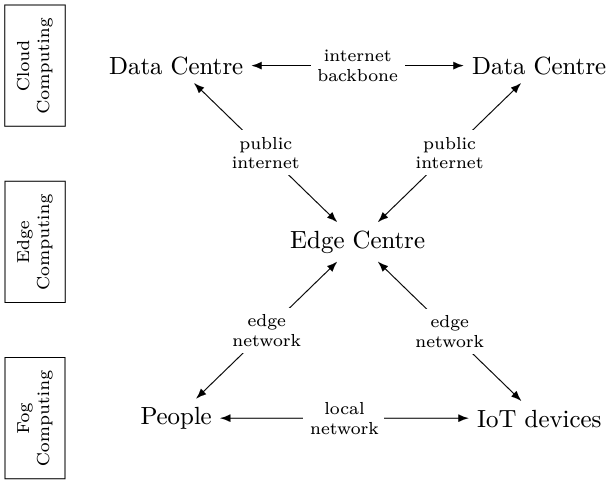
\includegraphics{images/edge_cloud_infrastructure.png}
	\caption[Panoramica sull'infrastruttura Edge Cloud]{Panoramica sull'infrastruttura Edge Cloud~\cite{berto_assurance-aware_2024}}\label{Edge cloud infrastructure}
\end{figure}

%Il continuum è il gestire sia cloud che edge come una cosa sola (in modo furbo)
In \cite{Cloud_Continuum} vengono raccolti 36 studi contenenti proposte di definizione per il \textbf{Cloud Continuum} e viene presentata come definizione complessiva \emph{``an extension of the traditional Cloud towards multiple entities (e.g., Edge, Fog, IoT) that provide analysis, processing, storage, and data generation capabilities``}.
Applicando questa definizione all'\emph{edge cloud continuum} si va a definire \emph{edge} e \emph{cloud} come entità presenti gestite come un'unica componente.
Le maggiori problematiche che il Continuum incontra con l'integrazione di nodi Edge sono dovute alla forte distribuzione geografica a cui sono soggetti gli elementi del sistema.
Le diverse distanze fisiche tra i nodi e i data-center introducono una variabilità nelle prestazioni e nella latenza a seconda della localizzazione, rendendo più difficile la capacità dei \textit{service provider} di soddisfare determinati \gls{SLA} \cite{Edge_cloud_continuum_challenges}. %https://www.queenstrl.ca/uploads/4/6/3/1/4631596/extreme_edge_computing_challenges_on_the_edge_cloud_continuum.pdf
I nodi edge richiedono anche opportune verifiche di proprietà di sicurezza e privacy, verificabili con maggiori sforzi, in quanto coinvolgono infrastrutture di terze parti.
Sorgono inoltre difficoltà nel mantenere la coerenza tra i dati in un ambiente così distribuito, vengono infatti richiesti protocolli sofisticati di sincronizzazione tra i data-center e i nodi edge che possano gestire eventuali conflitti o incongruenze derivanti dalla latenza della rete, la quale può provocare la ricezione di dati \textit{obsoleti} che comprometterebbero lo stato del sistema, e dall'elaborazione locale (dati elaborati localmente prima di essere sincronizzati col cloud). Ogni nodo possiede risorse computazionali e di storage differenti e limitate, questa eterogeneità fisica accentua la complessità nel sincronizzarsi in quanto i meccanismi e i protocolli da implementare dovranno adattarsi dinamicamente alle risorse dei vari nodi.

Nell'ambito delle infrastrutture distribuite moderne, l'Edge-Cloud Continuum rappresenta un paradigma emergente che unisce le capacità del cloud computing con l'elaborazione e l'archiviazione dati agli estremi della rete (\emph{edge computing}), il tutto in un'unico sistema complessivo (\emph{continuum}). Offre una piattaforma flessibile e scalabile che consente di distribuire le risorse computazionali tra cloud centralizzati e nodi edge situati più vicini agli utenti finali e ai dispositivi \gls{IoT}, comportando una gestione di entità distribuite geograficamente nel territorio.

Un sistema distribuito così complesso necessita tuttavia di un'adeguata soluzione per il monitoring e la verifica del suo corretto funzionamento. La natura eterogenea e geograficamente distribuita di un'infrastruttura Edge-Cloud richiede strumenti che possano garantire l'ottenimento di metriche da tutti i nodi del sistema per valutarne il relativo comportamento e rilevare anomalie o guasti, ottenendo così una soluzione di monitoring efficace.

\section{Monitoring}
In un sistema distribuito, l'affidabilità e le prestazioni dipendono dalla coordinazione e dall'integrità delle varie parti che lo compongono, rendendo il monitoraggio una pratica essenziale per garantire il corretto funzionamento dell'intero sistema. \\
Il monitoring è quella tecnica che si concentra sulla collezione di \emph{evidence}, o prove, per stabilire lo stato di salute e il comportamento del sistema. \\
Si basa su \textit{tre} elementi fondamentali:
\begin{itemize}
	\item \textbf{Logs}: registrazioni testuali di eventi che si verificano all'interno di un applicazione o di un sistema; possono includere errori, avvisi, informazioni operative e dati diagnostici. Sono informazioni strutturate in modo \textit{human-readable} in quanto pensate per essere analizzate manualmente. La gestione di grandi volumi di log provenienti da molteplici sorgenti è un problema che spesso trova soluzione nell'utilizzo di formati \textit{machine-readable} che permettono l'automatizzazione del processo di analisi.
	\item \textbf{Traces}: forniscono una visione dettagliata del percorso (\textit{trace}) che una richiesta segue in un sistema, salvando sia lo stato attuale che il relativo contesto di esecuzione. Ogni traccia è costituita da una serie di segmenti detti \textit{span} che rappresentano singole operazioni.
	\item \textbf{Metrics}: dati quantitativi che descrivono lo stato e le prestazioni di un sistema nel tempo. Includono informazioni come l'utilizzo della CPU, la memoria disponibile, il numero di richieste per secondo, la latenza delle risposte etc. Fondamentali per il monitoraggio in tempo reale e l'ottimizzazione delle prestazioni, offrono una panoramica immediata dello stato di salute del sistema.
\end{itemize}

Logs, traces e metrics sono strumenti complementari nel monitoraggio dei sistemi. Mentre i \emph{logs} forniscono un registro dettagliato degli eventi, le \emph{traces} permettono il tracciamento delle operazioni legate ad uno specifico evento a vari livelli e le \emph{metrics} consentono una misura oggettiva dello stato interno di un sistema, misure alla base della verifica di \emph{\glspl{PNF}}, approfondite nella Sezione \ref{Proprietà Non Funzionali}.

%https://www.researchgate.net/publication/3282450_Monitoring_distributed_systems#full-text
%https://dl.acm.org/doi/10.1145/13677.22723

%FORSE IL PI§ UTILE E RECENTE
%https://www.sciencedirect.com/science/article/pii/S1567832613000234

%https://ieeexplore.ieee.org/abstract/document/5557986
%https://www.sciencedirect.com/science/article/pii/S0030402615017271?casa_token=Kh33hZZHNYMAAAAA:fkpfBQJJlD3qNaCnKBY6X5OZYSNpzf-XPuEnD89EiOZ7qKiITUe0lqhGnH-XY_F9y5ZYbnHlzx8I

I primi sistemi di monitoring realizzati basati su metriche erano \textit{collettori di metriche \gls{SNMP}} il cui funzionamento è basato su un'applicazione centrale che interroga gli agenti \gls{SNMP} installati in ogni dispositivo per ottenere i dati raccolti e successivamente analizzarli. \'E un modello di monitoring completamente centralizzato e ormai superato.
La realizzazione di un sistema di monitoring attuale, invece, pone di fronte a varie scelte in merito all'architettura che il sistema andrà ad implementare, ciascuna caratterizzata da specifiche peculiarità. Alcuni esempi di scelte progettuali riguardano sia l'\textit{architettura} che l'applicativo di monitoring andrà ad avere, che l'effettivo procedimento di \textit{estrazione delle informazioni}.

\subsection{Architettura di monitoring e relative applicazioni}
Vengono analizzati alcuni esempi di tipiche architetture presenti nel mercato.
\begin{itemize}
	\item \emph{\textbf{Sistemi Completamente Centralizzati}}: sia la raccolta dei dati che il loro storage avvengono in un singolo punto centralizzato dove vengono in seguito processati e analizzati. Questo approccio fornisce semplicità, consistenza e affidabilità. Fornisce anche maggiore sicurezza e privacy in quanto i dati sono custoditi e processati in un unico ambiente. Dall'altro lato questo approccio causa alcuni svantaggi come un elevato sovraccarico del traffico di rete verso il nodo centrale e una limitata scalabilità.
	      Graylog\footnote{\label{graylog}\url{https://graylog.org/}} adotta questa architettura.

	\item \emph{\textbf{Sistemi Distribuiti}}: permettono di monitorare consistentemente i dispositivi nella rete raccogliendone le relative metriche. La raccolta ed elaborazione distribuita dei dati può ridurre la quantità di dati che devono essere trasmessi, il che può far risparmiare risorse di rete e migliorare l'efficienza. Viene inoltre migliorata la scalabilità.

	      \begin{itemize}
		      \item \emph{\textbf{Raccolta Distribuita ma Storage Centralizzato}}: i dati vengono raccolti da vari agenti o nodi distribuiti, ma vengono inviati a un punto centrale per lo storage e l'analisi. Alcuni servizi che si basano su questa architettura sono Prometheus\footnote{\label{prometheus}\url{https://prometheus.io/}} e Logstash\footnote{\url{https://www.elastic.co/logstash}}.

		      \item \emph{\textbf{Completamente Distribuito}}: sia la raccolta che lo storage dei dati sono distribuiti tra più nodi. I dati vengono memorizzati e processati in vari punti della rete, spesso con meccanismi di replica e bilanciamento del carico.
		            Alcuni servizi che si basano su questa architettura sono Elasticsearch\footnote{\label{elastic}\url{https://www.elastic.co/elasticsearch}} e Kafka\footnote{\url{https://kafka.apache.org/}}.
	      \end{itemize}
\end{itemize}

\subsection{Estrazione informazioni}\label{estrazione inforamzioni}
Un aspetto cruciale della progettazione è rappresentato dalle modalità con cui i dati o informazioni vengono estratti dai sistemi monitorati e trasferiti al sistema di raccolta e analisi. Le due modalità principali che permettono al sistema di monitoring di ottenere questi dati sono il \emph{pull} e il \emph{push}.
\begin{itemize}
	\item \textbf{Pull}: in questa modalità il sistema di monitoring richiede attivamente (\textit{polling}) i dati ai sistemi che sta monitorando; le metriche possono essere esposte sia dall'applicazione stessa (\textit{monitoring nativo}) che da \textit{agenti}, i quali si occupano di ottenere preventivamente le misurazioni.
	      \'E a tutti gli effetti una richiesta esplicita da parte del monitor verso gli \textit{endpoint} del sistema target. Un'esempio applicativo che segue questo paradigma è Prometheus\footref{prometheus}
	\item \textbf{Push}: in questa modalità il sistema di monitoring si aspetta di ricevere i dati su un interfaccia configurata per poterli elaborare; è il sistema monitorato ad inviare attivamente informazioni. Le metriche possono arrivare sia direttamente dall'applicazione che da agenti esterni. Un'esempio di applicativi che seguono questo paradigma sono Graylog\footref{graylog} e Elasticsearch\footref{elastic}
\end{itemize}

Come accennato nell'elenco, un altro aspetto legato al reperimento delle metriche riguarda la distinzione tra \emph{monitoring nativo}, detto anche \textit{agent-less}, e monitoring tramite \emph{agenti esterni}, detto \textit{agent-based}.
\begin{itemize}
	\item \textbf{Agent-based}: è una tecnica di monitoraggio che richiede l'installazione di un software, chiamato \emph{agente}, su ogni dispositivo da monitorare il quale è in grado di raccogliere e collezionare dati. Come descritto prima può essere configurato per interagire con un sistema che lavora in pull o push, rispettivamente risponde alle richieste che gli vengono fatte oppure invia autonomamente i dati. Questa metodologia, con gli adeguati permessi concessi all'agente, fornisce informazioni dettagliate sul sistema ma, dall'altro lato, utilizza un numero di risorse notabile nella macchina host e fornisce un possibile vettore di attacco aggiuntivo. Fornisce anche resilienza a problemi di rete in quanto un agente salva localmente le metriche rilevate.

	\item \textbf{Monitoring nativo o trasparente}: in questa tecnica non è necessaria l'installazione di nessun client per la raccolta dei dati sul dispositivo da monitorare ma si utilizzano strumenti e tecnologie di monitoraggio direttamente forniti all'interno delle applicazioni, evitando installazioni e configurazioni aggiuntive.
	      L'applicazione autonomamente raccoglie le proprie metriche e le espone secondo una delle modalità precedentemente elencate: può inviarle periodicamente (\emph{push}) oppure attendere di essere interrogata (\emph{pull}).
	      \'E più semplice da configurare e comporta un impatto significativamente inferiore sulle risorse del sistema host rispetto alla controparte con agenti; richiede tuttavia l'apertura di porte specifiche e dipende fortemente dalla qualità della connessione per effettuare il polling attivo dei dati.
\end{itemize}

%se no lo metto come \paragraph{}
\subsubsection{Formati e protocolli standard}\label{standard}
L'obbiettivo di ricercatori e sviluppatori è quello di utilizzare \emph{formati e protocolli standard} sia per lo scambio di dati che per la comunicazione.
Vengono garantite importanti proprietà come l'\emph{interoperabilità} tra diversi sistemi, prodotti e servizi permettendone la cooperazione senza problemi; \emph{sicurezza}, \emph{qualità} e \emph{performance} sono dovuti alle innumerevoli ricerche e utilizzi a cui una tecnologia viene sottoposta prima di essere definita standard. Altri pregi dovuti all'uso di standard sono la riduzione dei costi, sia di sviluppo che tecnologici, e la conformità legislativa ovvero il rispetto di \emph{standard legislativi} imposti.

Per integrare applicazioni e sistemi di monitoring in modo efficiente, si fa dunque largo uso di formati e protocolli standard. L'adozione di tecnologie consolidate, come l'uso di \gls{API} REST con body in formato JSON o di protocolli di rete standard come \gls{SNMP} o \emph{Syslog}, utilizzato per trasmettere e raccogliere semplici informazioni di logging dai diversi dispositivi della rete, facilita l'interoperabilità tra le applicazioni e i sistemi di monitoring, rendendo possibile l'invio e la ricezione di dati in modo standardizzato e leggibile.
Sono presenti anche standard imposti da applicativi o framework di monitoring \textit{open-source} come Prometheus\footref{prometheus} o OpenTelemetry\footnote{\url{https://opentelemetry.io/}} con il relativo \gls{OTLP} che rispettivamente trattano i dati come una time-series (flusso di valori con timestamp appartenenti alla stessa metrica) o come una struttura dati da loro definita (OpenTelemetry Model) (open-telemetry utilizza exporter che inviano i dati in  formato \gls{OTLP}, essendo uno standard viene supportato da vari servizi di monitoring come Prometheus, Jaeger, ecc).
Sono presenti anche standard per la trasmissione di metriche in ambienti \textit{cloud-native} come OpenMetrics\footnote{\url{https://openmetrics.io/}}.
Questa standardizzazione non solo semplifica l'integrazione e riduce la complessità di sviluppo, ma assicura anche una maggiore compatibilità tra diversi ambienti e piattaforme, migliorando l'efficienza operativa e la scalabilità del sistema.


\section{Proprietà Non Funzionali}\label{Proprietà Non Funzionali}
Per far fronte alle stringenti necessità di ottenere una visione sempre più completa sullo stato di un sistema sono state introdotte, al fianco delle proprietà funzionali, le \emph{\textbf{\glspl{PNF}}} il cui scopo è quello di definire \emph{come} il sistema svolge le sue funzioni concentrandosi su aspetti di \emph{qualità}, a differenza delle proprietà funzionali che definiscono \emph{cosa} effettivamente viene fornito.
Una \gls{PNF} di un sistema è un vincolo al modo in cui il sistema implementa e fornisce le sue funzionalità.
In altre pubblicazioni presenti in letteratura viene usato il termine \textit{Non Functional Requirements} riferendosi a \gls{PNF} con annesso il criterio di accettazione (requisito) da soddisfare; la metodologia adottata in questa tesi esprime formalmente i Non Functional Requirements e la loro verifica tramite Contratti, illustrati nella successiva Sezione \ref{assurance methodology}.

In questa pubblicazione \cite{review_microservices_NFR} vengono analizzati 36 paper aventi come topic le architetture a microservizi, tra questi 21 discutono le tecniche per verificare \textit{Non Functional Requirements}. La proprietà più discussa in letteratura risulta essere l'\emph{affidabilità}, seguita da \emph{scalabilità} e \emph{disponibilità}. \\
Di seguito vengono elencati e illustrati alcuni esempi di \emph{\glspl{PNF}} che possono essere misurate e valutate in un sistema.
\begin{itemize}
	%Definizioni ISO https://iso25000.com/index.php/en/iso-25000-standards
	\item \textbf{\textit{Reliability}}: affidabilità, capacità di funzionare correttamente e senza interruzioni per un determinato periodo di tempo, garantendo prestazioni stabili. \\
	Definizione ISO \cite{iso_system_quality} \textit{"Degree to which a system, product or component performs specified functions under specified conditions for a specified period of time"}.
	\item \textbf{\textit{Performance}}: prestazioni, capacità di un sistema di eseguire le sue funzionalità in modo efficiente rispettando dei requisiti e aspettative definiti dall'utente. \\
	Definizione ISO \cite{iso_system_quality} \textit{" the degree to which a product performs its functions within specified time and throughput parameters and is efficient in the use of resources (such as CPU, memory, storage, network devices, energy, materials...) under specified conditions"}.
	\item \textbf{\textit{Scalability}}: scalabilità, capacità di un sistema di gestire un aumento del carico di lavoro senza compromettere prestazioni o affidabilità. \\
	Definizione ISO \cite{iso_system_quality} \textit{"Degree to which a product can handle growing or shrinking workloads or to adapt its capacity to handle variability"}.
	\item \textbf{\textit{CIA - Confidentiality}}: confidenzialità, garantisce che i dati vengano acceduti solo da chi effettivamente autorizzato e non vengano divulgati. \\
	Definizione ISO \cite{iso_system_quality} \textit{"Degree to which a product or system ensures that data are accessible only to those authorized to have access"}.
	\item \textbf{\textit{CIA - Integrity}}: integrità, garantisce che i dati siano accurati, completi e non alterati in modo non autorizzato; in altre parole i dati sono corretti e attendibili. \\
	Definizione ISO \cite{iso_system_quality} \textit{"Degree to which a system, product or component ensures that the state of its system and data are protected from unauthorized modification or deletion either by malicious action or computer error"}.
	\item \textbf{\textit{CIA - Availability}}: disponibilità, il sistema è accessibile e operativo quando richiesto. \\
	Definizione ISO \cite{iso_system_quality} \textit{"Degree to which a system, product or component is operational and accessible when required for use"}.
	\item \textbf{\textit{Access control}}: controllo accessi, solo gli utenti autorizzati dalle politiche del sistema possono accedere alle risorse
	\item \textbf{\textit{Resilience}}: resilienza, capacità di un sistema di continuare a funzionare correttamente, e di recuperare rapidamente, in seguito ad un guasto. \\
	Definizione ISO \cite{iso_system_quality} \textit{"Degree to which a product can automatically place itself in a safe operating mode, or to revert to a safe condition in the event of a failure"}.
\end{itemize}

\'E importante sottolineare il fatto che queste proprietà definiscono degli obbiettivi concettuali da raggiungere ma non trattano le modalità con cui si verifica l'effettivo soddisfacimento. Questo accade perché le modalità di verifica differiscono in base all'entità che si sta controllando ed è compito di un \textit{esperto del sistema}, colui che ha adeguate conoscenze e competenze, andare a definire come una proprietà si può concretizzare in uno specifico contesto.
%cambiare definire
Gli esempi illustreranno come l'espressione pratica dello stesso concetto è strettamente legata al contesto di applicazione.

\begin{exmp}
	Valutando l'\textit{availability} di un server si misura il tempo durante il quale il server è \textit{up} e funziona correttamente (riceve le richieste e risponde fornendo il relativo servizio) mentre valutando l'\textit{availability} di una rete cellulare si va a misurare la capacità della rete di fornire connessione ai dispositivi mobili in una determinata area geografica.
\end{exmp}

\begin{exmp}
	Valutando l'\textit{Integrity} di una comunicazione di rete ci si riferisce alla capacità di trasmettere e ricevere i dati senza alterazioni o perdite mentre valutando l'\textit{Integrity} di uno \textit{storage} (come un database o un dispositivo di archiviazione fisico) ci si riferisce alla capacità di garantire che i dati archiviati non vengano alterati e rimangano completi.
\end{exmp}

\section{Verifica di Proprietà non Funzionali - Assurance}\label{Verifica di PNF}
Le tecniche di \textbf{assurance} mirano a garantire che un sistema \emph{verifichi}, e quindi soddisfi, determinate Proprietà Non Funzionali precedentemente definite. \\
Per questa tesi viene adottata la \emph{\textbf{metodologia di assurance}} utilizzata in \cite{berto_assurance-aware_2024}, e riportata in questa sezione, che si occupa di misurare e valutare \glspl{PNF} di un'infrastruttura target sulla base delle \textit{evidence} raccolte dagli endpoint di monitoring. La verifica viene formalizzata attraverso l'uso di contratti basati sulle \textit{evidence} raccolte.
Questa metodologia adottata per il processo di \emph{assurance} mira a valutare un sistema indipendentemente dallo stato in cui si trova durante la valutazione (valutazione statica) basando i suoi risultati su misurazioni raccolte, archiviate in uno storage e indicizzate nel tempo invece che su misure dirette, permettendo così la definizione di contratti basati su intervalli temporali.

Ogni componente del sistema possiede uno \emph{stato interno}, rappresentazione dinamica dello stato delle variabili e delle risorse, e una \emph{configurazione}, configurazione statica del componente che ne caratterizza il comportamento, utilizzati per valutarne determinate proprietà.
Questi due dati (stato interno e configurazione) vengono esposti dal componente del sistema al processo di assurance tramite interfacce di monitoring standard dette anche \emph{endpoint di monitoring}.
Gli endpoint andranno a rappresentare il target del processo di assurance per la raccolta di \textit{measurements} dall'infrastruttura.

\subsection{Assurance methodology}\label{assurance methodology}

\begin{figure}[th]
	\centering
	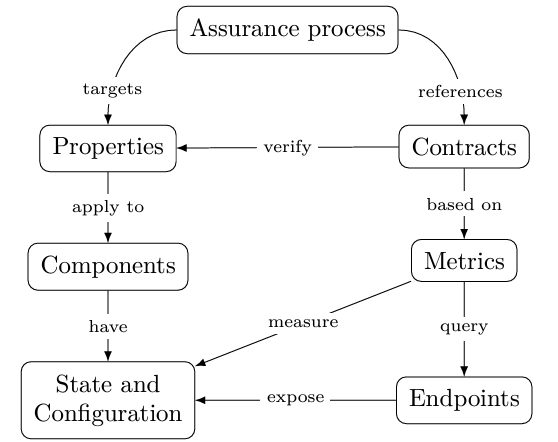
\includegraphics{images/assurance_methodology.png}
	\caption[Schema di \emph{assurance methodology}]{Schema di \emph{assurance methodology} proposto in~\cite{berto_assurance-aware_2024}}\label{Schema assurance methodology}
\end{figure}

La Figura \ref{Schema assurance methodology} mostra lo schema della metodologia di assurance che verrà utilizzato nel corso di questa tesi. \\
La metodologia adottata in \cite{berto_assurance-aware_2024} utilizza gli endpoint delle infrastrutture come fonte di misurazioni (espongono lo stato e le configurazioni del sistema).
Le misurazioni degli endpoint vengono valutate attraverso \textbf{metriche} le quali si focalizzano sulla valutazione di un comportamento specifico per verificare \glspl{PNF}.
Le metriche, una volta valutate e ottenute le relative \textit{evidence}, diventano la base per la valutazione dei \textbf{contratti}, i quali fanno riferimento direttamente a una \gls{PNF} specifica e descrivono come può essere verificata in modo formale.
Individuiamo nelle \emph{metriche} e nei relativi \emph{contratti} gli elementi focali di questa sezione.

\paragraph{Metriche}
Una metrica è una funzione associata da una funzionalità, la quale vuole misurare i suoi aspetti o comportamenti sui componenti che la implementano; è un \textit{qualsiasi tipo di trasformazione che viene applicato ai dati} per trasformarli in una forma più utile. La più semplice trasformazione, definita identità, consiste nel tenere i dati grezzi ``così come sono``.
Esistono poi trasformazioni che vanno a ridurre la quantità di dati raccolti rispetto al totale reperibile dal sistema, mirando ad estrarre proprietà o informazioni specifiche da essi.
Vengono definite sugli stati e sulle configurazioni esposte dagli endpoint di monitoring. La valutazione delle metriche fornisce le \textit{\textbf{evidence}}, o prove, misurazione oggettive atte a confermare se una particolare proprietà è valida.

\paragraph{Contratti}
Descrivono formalmente come validare le proprietà di un servizio. Un contratto è una funzione booleana il cui scopo è quello di valutare la validità o meno di una determinata proprietà. La valutazione avviene basandosi sulle \textit{evidence}, o prove, ottenute tramite valutazione delle metriche degli endpoint.
Un contratto è una tupla costituita dal \emph{istante di tempo} in cui è avvenuta la valutazione e dal \emph{set di componenti} che implementano il servizio target.
Un aspetto cruciale dei contratti è essere \textit{time-dependant}, l'esito dipende quindi dall'istante temporale in cui è stato valutato il contratto.
Per garantire consistenza, questa metodologia mira a definire un solo contratto per ogni proprietà (mapping bigettivo tra proprietà e contratto).

\subsection{Assurance process}\label{assurance process}
\begin{figure}[th]
	\centering
	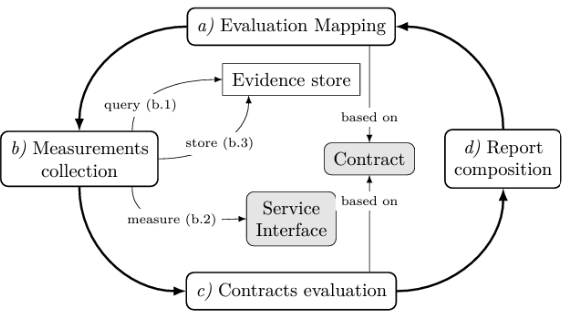
\includegraphics{images/assurance_process.png}
	\caption[Schema di \emph{assurance process}]{Schema di \emph{assurance process} proposto in\cite{berto_assurance-aware_2024}}\label{Assurance process}
\end{figure}
%https://ieeexplore.ieee.org/stamp/stamp.jsp?tp=&arnumber=9750109
Un processo di assurance dipende da una \emph{assurance methodology} per validare le proprietà.
La soluzione adottata in \cite{berto_assurance-aware_2024} supporta la verifica continua e collaborativa di \glspl{PNF} delle componenti infrastrutturali.
La Figura \ref{Assurance process} applica l'\emph{assurance methodology} vista nella Sezione \ref{assurance methodology} suddividendo il processo in 4 step ripetuti ciclicamente.
\begin{enumerate}[label=(\alph*)]
	\item \emph{Evaluation mapping}: nel primo step, partendo dalle \emph{proprietà} che si intendono verificare si va ad identificare le \emph{metriche} e i \emph{contratti} che dovranno essere valutati per poter effettuare quegli accertamenti

	\item \emph{\textbf{Measurement} collection}: il passo successivo consiste nella valutazione  delle metriche (\textit{metrics evaluation}) precedentemente identificate e fornite dal servizio, step b.2, e nella seguente raccolta e immagazzinamento delle \textit{evidence} generate (\textit{measurements}), step b.3.

	\item \emph{\textbf{Contracts} evaluation}: nel terzo passaggio viene eseguita l'effettiva verifica delle proprietà, calcolando il risultato del \emph{contratto}, utilizzando le misurazioni raccolte in precedenza (\textit{measurements} usate come \textit{evidence} per comprovare un contratto) e restituendo un output booleano.

	\item \emph{Report composition}: nell'ultimo passaggio i risultati parziali, \emph{measurements} e \emph{contracts evaluation}, vengono aggregati in un report che include una descrizione dei risultati (proprietà verificate o no) e le relative \textit{evidence} a supporto. Il report viene generato seguendo un formato \textit{machine readable} per garantirne il facile utilizzo in altri processi automatizzati, come la certificazione descritta nella sezione successiva.
\end{enumerate}


\section{Certificazione di Proprietà non Funzionali - Certification}
La \textbf{certificazione} è una tecnica di \textit{security assurance} il cui scopo è dimostrare, seguendo uno \emph{schema di certificazione}, che un sistema target, in un determinato istante di tempo, si comporti come previsto e soddisfi determinate \glspl{PNF}. Il funzionamento è costituito in parte dalla \emph{verifica di \glspl{PNF}} precedentemente illustrata nella Sezione \ref{Verifica di PNF} ma con l'aggiunta di una \gls{CA} il cui compito è la gestione sicura del processo di verifica garantendo sicurezza, affidabilità e ripetibilità.
La certificazione, come menzionato in \cite{certification_sw_development}, è stata integrata nel ciclo di vita dei sistemi distribuiti, partendo dallo sviluppo degli stessi, per aumentare la qualità del servizio e garantire un comportamento stabile nel tempo.

\begin{figure}[th]
	\centering
	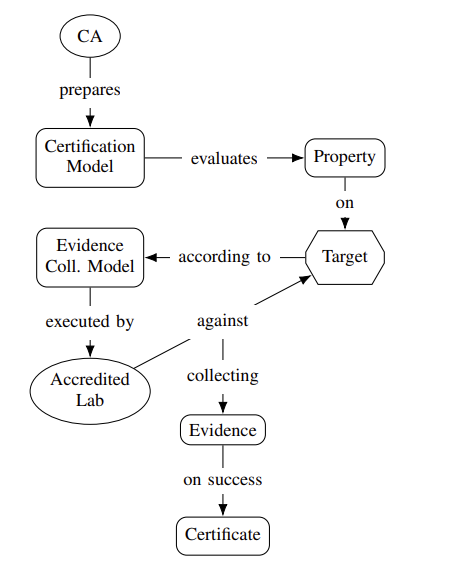
\includegraphics{images/certification_process}
	\caption[Generico processo di certificazione]{Generico processo di certificazione~\cite{NF_certification_distributed_system}}\label{Generico processo di certificazione}
\end{figure}

%vedi questa citazione https://dl.acm.org/doi/10.1145/2767005

Per questa tesi viene adottata la metodologia menzionata in Ardagna et al.\ \cite{NF_certification_distributed_system} utilizzando la loro nomenclatura.
La Figura \ref{Generico processo di certificazione} mostra un generico schema di certificazione contenente le entità coinvolte (\gls{CA}, \gls{AL} e Target) e le varie interazioni per giungere ad un certificato. \'E fondamentale la creazione di una \textit{chain-of-trust} tra l'\textit{utente} che chiede la certificazione, la \gls{CA} che prepara il \textit{certification model}, l'\gls{AL} che esegue il \textit{certification model} e il certificato rilasciato.
Segue un'illustrazione delle componenti presenti nello schema.

\paragraph{Target}
rappresenta l'obbiettivo del processo di certificazione ed è costituito dalle implementazioni concrete dei componenti del sistema a cui il certificato è rivolto (un software, un servizio o un sistema in senso più ampio).

\paragraph{\gls{CA}}
Ha il compito di definire e orientare tutte le attività necessarie per valutare e certificare una specifica proprietà su un Target; lo fa definendo un \emph{Certification Model} che contiene un \emph{Evidence Collection Model}.
Fornisce delle linee guida fondamentali per assicurare che il processo di certificazione sia condotto in modo sistematico e conforme ai requisiti predefiniti garantendo sicurezza e affidabilità.

\subparagraph{Certification Model}
Una specifica delle attività da eseguire per certificare \glspl{PNF} sul sistema target.
Il modo più conciso di rappresentarlo è una tupla costituita da \emph{Proprietà} che si intendono verificare, \emph{Target} ed \emph{Evidence Collection Model}. \'E parte fondamentale di un certificato in quanto definisce cosa si sta certificando (proprietà), come (\emph{evidence collection model}) e chi si sta certificando (target) andando a definire concretamente come deve avvenire la certificazione.

\subparagraph{Evidence}
tutti i dati raccolti e valutati i modo oggettivo su un sistema target, include sia i dati delle metriche che le valutazioni fatte

\subparagraph{Evidence Collection Model}
coordina le attività necessarie a raccogliere \textit{evidence} dal sistema target, le quali verranno valutate per stabilire il rilascio del certificato o meno.
Definisce come i dati raccolti dal sistema di monitoring vanno all'\gls{AL}.

\paragraph{\gls{AL}}
sono laboratori riconosciuti ufficialmente da un ente di accertamento e richiedono di rispettare determinate norme (ad esempio \textit{\cite{iso_testing}: General requirements for the competence of testing and calibration laboratories}) per garantire affidabilità e precisione dei risultati.
Viene delegato dalla \gls{CA} per eseguire l'\emph{Evidence Collection Model} sul sistema target; con i dati raccolti, le \textit{evidence}, il laboratorio potrà assegnare un certificato al sistema in caso di valutazione positiva %vedi citazione https://ieeexplore.ieee.org/document/9844845


\paragraph{Certificato}
il certificato viene rilasciato dalla CA ai sistemi target che superano con successo la valutazione di determinate \glspl{PNF} sulla base delle \emph{evidence} raccolte, ne attesta la conformità. Contiene un riferimento al \textit{certification model}, il quale ne illustra i dettagli, e alle \textit{evidence} raccolte che ne supportano la validità.

\paragraph{Flusso di esecuzione:} La \gls{CA} definisce il \emph{Certification Model} costituito dalle proprietà che devono essere verificate su un sistema target seguendo uno specifico \emph{Evidence Collection Model}. L'\gls{AL}, delegato dalla \gls{CA}, ha l'incarico di raccogliere le prove o \textit{evidence} dal sistema.
Se le \emph{evidence} dimostrano positivamente la conformità della proprietà viene rilasciato un \emph{certificato} che attesta la conformità del sistema ai requisiti stabiliti.


\section{Related Work}
%In [] viene proposta una metodologia basata su ... il cui scopo è ... \\
%(2014)
In \cite{Multi_layer_Cloud_Assurance_Evaluation_methodology} viene proposta una metodologia di valutazione multi-layer (monitora il livello fisico, le VM e le applicazioni in esecuzione sulle VM raccogliendo metriche a vari livelli di granularità) e continua, fondata sui \gls{CC}\footnote{https://www.commoncriteriaportal.org/}, per valutare i livelli di sicurezza delle applicazioni Cloud, in termini di Assurance Level, attraverso l'aggregazione delle proprietà di sicurezza, raccolte su vari livelli, dei singoli componenti che le costituiscono.
Fornisce al proprietario del servizio una panoramica della sicurezza del suo servizio senza la necessità di analisi manuali dettagliate.

%(2016)
In \cite{certification_cloud_services} viene proposto un framework di certificazione della sicurezza test-based (test-based assurance: le evidence arrivano da test e non da strumenti di monitoring) per servizi cloud.
Fornisce una metodologia e un ambiente di cloud-engineering basati su certificati con il relativo set di componenti che gestisce il processo di certificazione, online e semi-automatico, di servizi/applicazioni in un sistema cloud-based; fornisce anche dei tools in supporto alla chain-of-trust imposta dalla certificazione.
Il framework infine supporta la valutazione di sistemi cloud sia pre-deployment che in production-deployment a diversi livelli, discostandosi dai tradizionali strumenti che non considerano il processo di sviluppo.

%(2020)
In \cite{semiautomatic_continuous_cloud_certification} viene proposta una rigorosa e adattiva tecnica di assurance basata sulla certificazione che mira ad un ecosistema cloud trasparente ed affidabile dove ogni parte del cloud si comporta come previsto.
Utilizza uno schema di certificazione basato su test per dimostrare il soddisfacimento di \gls{PNF} dei servizi cloud; una \gls{CA}, online e disponibile durante l'intero processo, definisce i requisiti non funzionali da verificare su un determinato modello. Il controllo avviene in modo semi-automatico tramite un algoritmo di matching che effettua un confronto tra il certification model definito dalla CA e un'istanza.
Presenta inoltre un processo continuo e incrementale di gestione del ciclo di vita di un certificato (semi-)automatico, dall'emissione al suo riadattamento a cambi contestuali (cloud multilayer dinamici) alla revoca.
Il framework è stato applicato in uno scenario industriale reale per la gestione di un sistema di pagamento (ENGpay) e ne sono state valutate prestazioni, qualità, applicabilità e usabilità pratica.
%OPTIONAL TODO
%\hl{
%posso collegarlo alla citazione sopra dicendo che è un paper specifico che parla dei cambi nei sistemi (questo è del 2023 quello sopra del 2020 quindi ha senso)
%https://air.unimi.it/handle/2434/1018841: Continuous Certification of Non-functional Properties Across System Changes
%}

%(2021)
In \cite{assurance_risk_managament_ds} viene proposto un framework di gestione del rischio per sistemi distribuiti basato su tecniche di \emph{assurance}, le quali monitorano il comportamento del sistema tramite valutazione di \gls{PNF}, che soddisfa i requisiti di \emph{gestione del rischio} imposti dai moderni sistemi distribuiti; statistiche come performance e qualità del framework sono state misurate in uno scenario simulato di industria 4.0.
Questo framework fornisce un espansione ai framework di risk-management consentendo alle organizzazioni grandi e complesse di valutare il proprio rischio basandosi su risultati derivanti dalla valutazione di \gls{PNF} relativi all'efficacia dei meccanismi implementati, integrando quindi completamente il concetto di \emph{assurance} alla gestione del rischio.

In questi due paper vengono proposti studi in merito all'\textbf{assurance in dispositivi \gls{IoT}} le cui ricerche rispetto a servizi e sistemi cloud sono ancora agli inizi. \\
%(2021)
In \cite{assurance_framework_edge_iot} viene proposto un framework altamente automatizzato di security assurance per sistemi Edge e \gls{IoT}, paradigmi di elaborazioni emersi negli ultimi anni, indipendente dalle complessità infrastrutturali e basato su un'architettura di Kubernetes avanzata in grado di gestire applicazioni 5G-native.
Implementa un processo di assurance altamente scalabile che garantisce la verifica di \gls{PNF} raccogliendo evidence dal sistema target.
Come caso reale di applicazione viene presentato l'\gls{IoMT} considerano come contesto di esecuzione un moderno ospedale dotato di molti device eterogenei (sensori umidità e temperatura, dispositivi \gls{IoT} medici ecc). \\
%(2022)
L'anno successivo in \cite{assurance_iot} il framework proposto in precedenza viene ampliato introducendo il concetto di assurance \gls{IoT} guidata da una visione olistica del sistema di destinazione.
Questo metodo definisce ed esegue valutazioni di assurance che si allineano e sfruttano l'architettura del sistema target, distribuendo e aggregando i calcoli di conseguenza.
Il framework considera l'intero ciclo di vita del sistema e produce risultati a diversa granularità attraverso una valutazione di assurance basata su attività multi-layer, multifase (in diversi momenti del suo ciclo di vita) e comportamentali.
Il framework proposto è stato valutato in uno \emph{Smart Light System} reale.

%(2023)
Come visto in \cite{NF_certification_distributed_system}, la certificazione di moderni sistemi distribuiti incontra alcune \emph{difficoltà} dovute sia al continuo adattamento ed evoluzione dei sistemi, implicando l'invalidamento dei corrispondenti certificati (la cui realizzazione richiede sforzo in termini di tempo e risorse), che alla presenza di \gls{ML} a livello applicativo e infrastrutturale. Queste caratteristiche rendono il comportamento del sistema impredicibile, in contrasto con i principi fondanti della certificazione quali \emph{staticità, predicibilità e verificabilità}.


%TOP spiegazione certificazione
%(2023)
Lo schema di certificazione proposto in \cite{multi_dimensional_certification_ds} va oltre la semplice valutazione del comportamento di un servizio, prendendo in considerazione fattori aggiuntivi che descrivono, ad esempio, come il servizio è stato implementato e verificato, con l'obiettivo di aumentare la qualità e le prestazioni di un sistema distribuito.
Questo approccio è definito certificazione multidimensionale, poiché include dimensioni aggiuntive che modellano aspetti rilevanti (ad esempio, linguaggi di programmazione e processi di sviluppo) che contribuiscono in modo significativo alla qualità dei risultati della certificazione; l'obiettivo non si limita più alla valutazione delle \gls{PNF} degli artefatti software ma viene esteso per considerare \emph{dimensioni} aggiuntive, come ad esempio i processi di sviluppo e verifica.
Questo schema certifica le proprietà di un dato servizio considerando ogni dimensione in modo indipendente:
compone i risultati della valutazione in ogni dimensione e produce un certificato accurato del comportamento del servizio.
Lo schema infine è integrato nella gestione del ciclo di vita (dallo sviluppo del sistema al suo funzionamento e alla sua manutenzione) di sistemi distribuiti per supportare una selezione dei servizi basata sulla certificazione, in cui i servizi funzionalmente equivalenti vengono classificati (service ranking) in base alle \gls{PNF} certificate che detengono e ai requisiti degli utenti corrispondenti, utilizzando una tecnica di Multi-Criteria Decision-Making (MCDM).
Questa modellazione porta a certificati più accurati e, di conseguenza, a un processo decisionale più accurato quando i servizi/software vengono selezionati dinamicamente in fase di esecuzione sulla base dei loro certificati. \\
In conclusione questo approccio offre vantaggi per tutte le parti coinvolte: i fornitori di servizi ottengono certificati che riflettono meglio tutte le best practice seguite; gli utenti finali possono fare scelte più consapevoli grazie a certificati dettagliati e ben strutturati; la CA fornisce uno schema di certificazione più utile.


%https://air.unimi.it/retrieve/dfa8b99d-09e9-748b-e053-3a05fe0a3a96/main.pdf : Test-Based Security Certification of Composite Services


%https://air.unimi.it/handle/2434/554823: "Certification-Based Cloud Adaptation"
%Ardagna et al. [136] described a lightweight certification methodology for cloud environments, supported by continuous monitoring of infrastructures, platforms and services.

%https://air.unimi.it/handle/2434/371230: Security certification for the Cloud: the CUMULUS approach

%https://air.unimi.it/handle/2434/921233: A security certification scheme for Information-Centric Networks: proposed a formal certification scheme to validate NFPs cloud-based services.

%https://air.unimi.it/retrieve/handle/2434/888053:
%“Security Certification Scheme for Content-centric Networks,
